%%% LaTeX Template: Article/Thesis/etc. with colored headings and special fonts
%%%
%%% Source: http://www.howtotex.com/

\documentclass[12pt]{article}


\usepackage{apuntes-estilo}
\usepackage{fancyhdr,lastpage}
\usepackage{color,colortbl}
\usepackage{verbatim}

\def\maketitle{

% Titulo 
 \makeatletter
 {\color{bl} \centering \huge \sc \textbf{
 Manteniendo la hora \\ 
\large \vspace*{-8pt} \color{black} Guia básica de reconocimiento y monitoreo de recursos. 
 \vspace*{8pt} }\par}
 \makeatother


% Autor
 \makeatletter
 {\centering \small 
 	Departamento de Ingeniería de Computadoras \\
 	Facultad de Informática - Universidad Nacional del Comahue \\
 	\vspace{20pt} }
 \makeatother

}

% Custom headers and footers
\fancyhf{} % clear all header and footer fields
\fancypagestyle{plain}{\fancyhf{}}
  	\pagestyle{fancy}
 	\lhead{\footnotesize Reconocimiento y monitoreo de recursos - Departamento de Ingeniería de Computadoras}
 	\rhead{\footnotesize \thepage\ }	% ''Page 1 of 2''

\def\ti#1#2{\texttt{#1} & #2 \\ }



\begin{document}

\thispagestyle{empty}
\maketitle
\setlength{\parindent}{0pt}

\section*{Introducción}

Un administrador de sistemas es quien administra los recursos de un sistema informático. El administrador
de sistemas debe conocer cuáles son los recursos a administrar: cómo identificarlos y verificar su 
correcto funcionamiento. Durante esta guía se verán una serie de comandos y procedimientos para identificar 
recursos y verificar su estado. Dada la variedad del hardware existente hoy en día, este apunte no pretende
ser exhaustivo sino plantear un método de identificación y monitoreo a partir de ejemplos. Cunado 
el recurso a administrar no este dentro de lo visto en esta guía el administrador deberá preguntarse e
investigar cuál es la forma de inentificar y observar el estado del recurso en cuestión. 

Cuando hablamos de recursos en general nos referimos a representaciones en el sistema operativo para 
recursos físicos, como por ejemplo un CPU. O bien a recursos netamente lógicos que no tienen una
contraparte física como puede ser un proceso (programa en ejecución), una prioridad de ejecución, 
un sistema de archivos, etc. 


\section*{Identificando recursos}

\subsection*{Identificando el hardware}
Comenzaremos por identificar recursos físicos. 

\subsection*{Identificando recursos netamente lógicos}

\section*{Monitoreo de recursos}

\begin{center}
 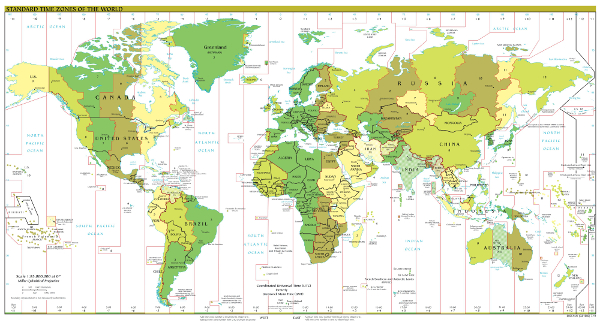
\includegraphics{World_Time_Zones_Map.jpg}
\end{center}

\colorbox{grey}{\parbox[t]{0.95\linewidth}{ \vspace*{0.5cm} { 
{\tt 
11) none - I want to specify the time zone using the Posix TZ format.\\
\#? 1\\
}
} \vspace*{0.5cm} } } 




\section*{Licencia}

Este material es una obra derivada de los siguientes textos:

``The Clock Mini-HOWTO'' del sitio TLDP: http://tldp.org/HOWTO/Clock.html\#toc1

``The Linux System Administrator's Guide'' del sitio TLDP: http://www.tldp.org/LDP/sag/html/

\end{document}
